\section{Hardware and Software platform}

In order to test the embedded implementation of MPC on real aircraft, one has to either use an existing platform or develop its own. Creating a custom hardware is a tedious job, but it is an investment that may eventually repay itself by providing complete control over platform's parameters and design. The key decision has been done to improve the existing design of custom control board (see thesis \citep{baca2013} for more details) emphasizing possibility to reuse the code that has been already developed. A new version has been designed by incorporating experience and observations from prior development. Following chapter firstly describes the UAV used for experimental validation of the control design, then there is the new control board presented with overview of its features and capabilities, and lastly the software structure is discussed including used realtime operating system and custom matrix library.

\subsection{UAV platform}

The UAV is a custom built tricopter (fig. \ref{fig:tricopter}) with one propeller mounted on a tilting mechanism. It has a capability to pitch, roll and yaw just as any other multirotor UAV. The yaw control is supplied by the tilting mechanism while pitch and roll can be controlled by changing the ratio between rotational speed of all motors. All propellers are mounted directly on brushless motors, each one of them controlled by an individual ESC (electronic speed controller). It it capable of lifting payload of $150 \jed{g}$ while its weight is $450\jed{g}$. Its flight time is 7 minutes on average. Propellers are $5\times3.8 \jed{inch}$ in dimensions, mounted on motors by rubber bands to increase safety.

The aircraft is equipped with the \textit{KK2} board which provides the basic stabilization of pitch and roll angles ($\theta$, $\psi$) and yaw rate ($\dot{\phi}$). It is a low-cost ($\approx 30\jed{USD}$) commercial product with open-source software. It utilizes 3-axis MEMS gyroscopes and accelerometers to estimate $\theta$, $\psi$, $\dot{\phi}$ and allow the vehicle to be controlled as an RC model. It incorporates a set of nested PID controllers for both attitude axis. They can be easily tuned using built-in display and buttons. It can handle various types of multirotor aircraft including the tricopter. Another important module is the \textit{px4flow} which is the only sensor used for localization in space (see section \ref{cap:px4flow} for more information).

\subsection{px4flow sensor}
\label{cap:px4flow}

The vehicle is localized in space by \textit{px4flow} sensor \citep{px4flow} (fig. \ref{fig:px4flow}), developed and produced by PixHawk \citep{pixhawk}. It encapsulates two sensors --- a camera for computing an optical flow and an ultrasonic rangefinder for measuring a distance from the ground. It provides an information about its velocity relative to the ground computed by the correlation of two consecutive images from the camera (the same principle as with most computer mice). The velocity is internally compensated from rotational motion by built-in gyroscope and finally scaled to absolute values using the altitude measured by the ultrasonic sensor. The sensor is able to measure velocities up to $0.5\jed{ms^{-1}}$ when flying in 1 meter altitude in good light conditions. The altitude is measured from $0.3\jed{m}$ to $4\jed{m}$. Data is sent in frequency around $70\jed{Hz}$ over UART (universal asynchronous receiver-transmitter) using MAVLink protocol \citep{px4flow}.

\begin{figure}[tbp]
\centering

\begin{subfigure}[b]{0.55\textwidth}
	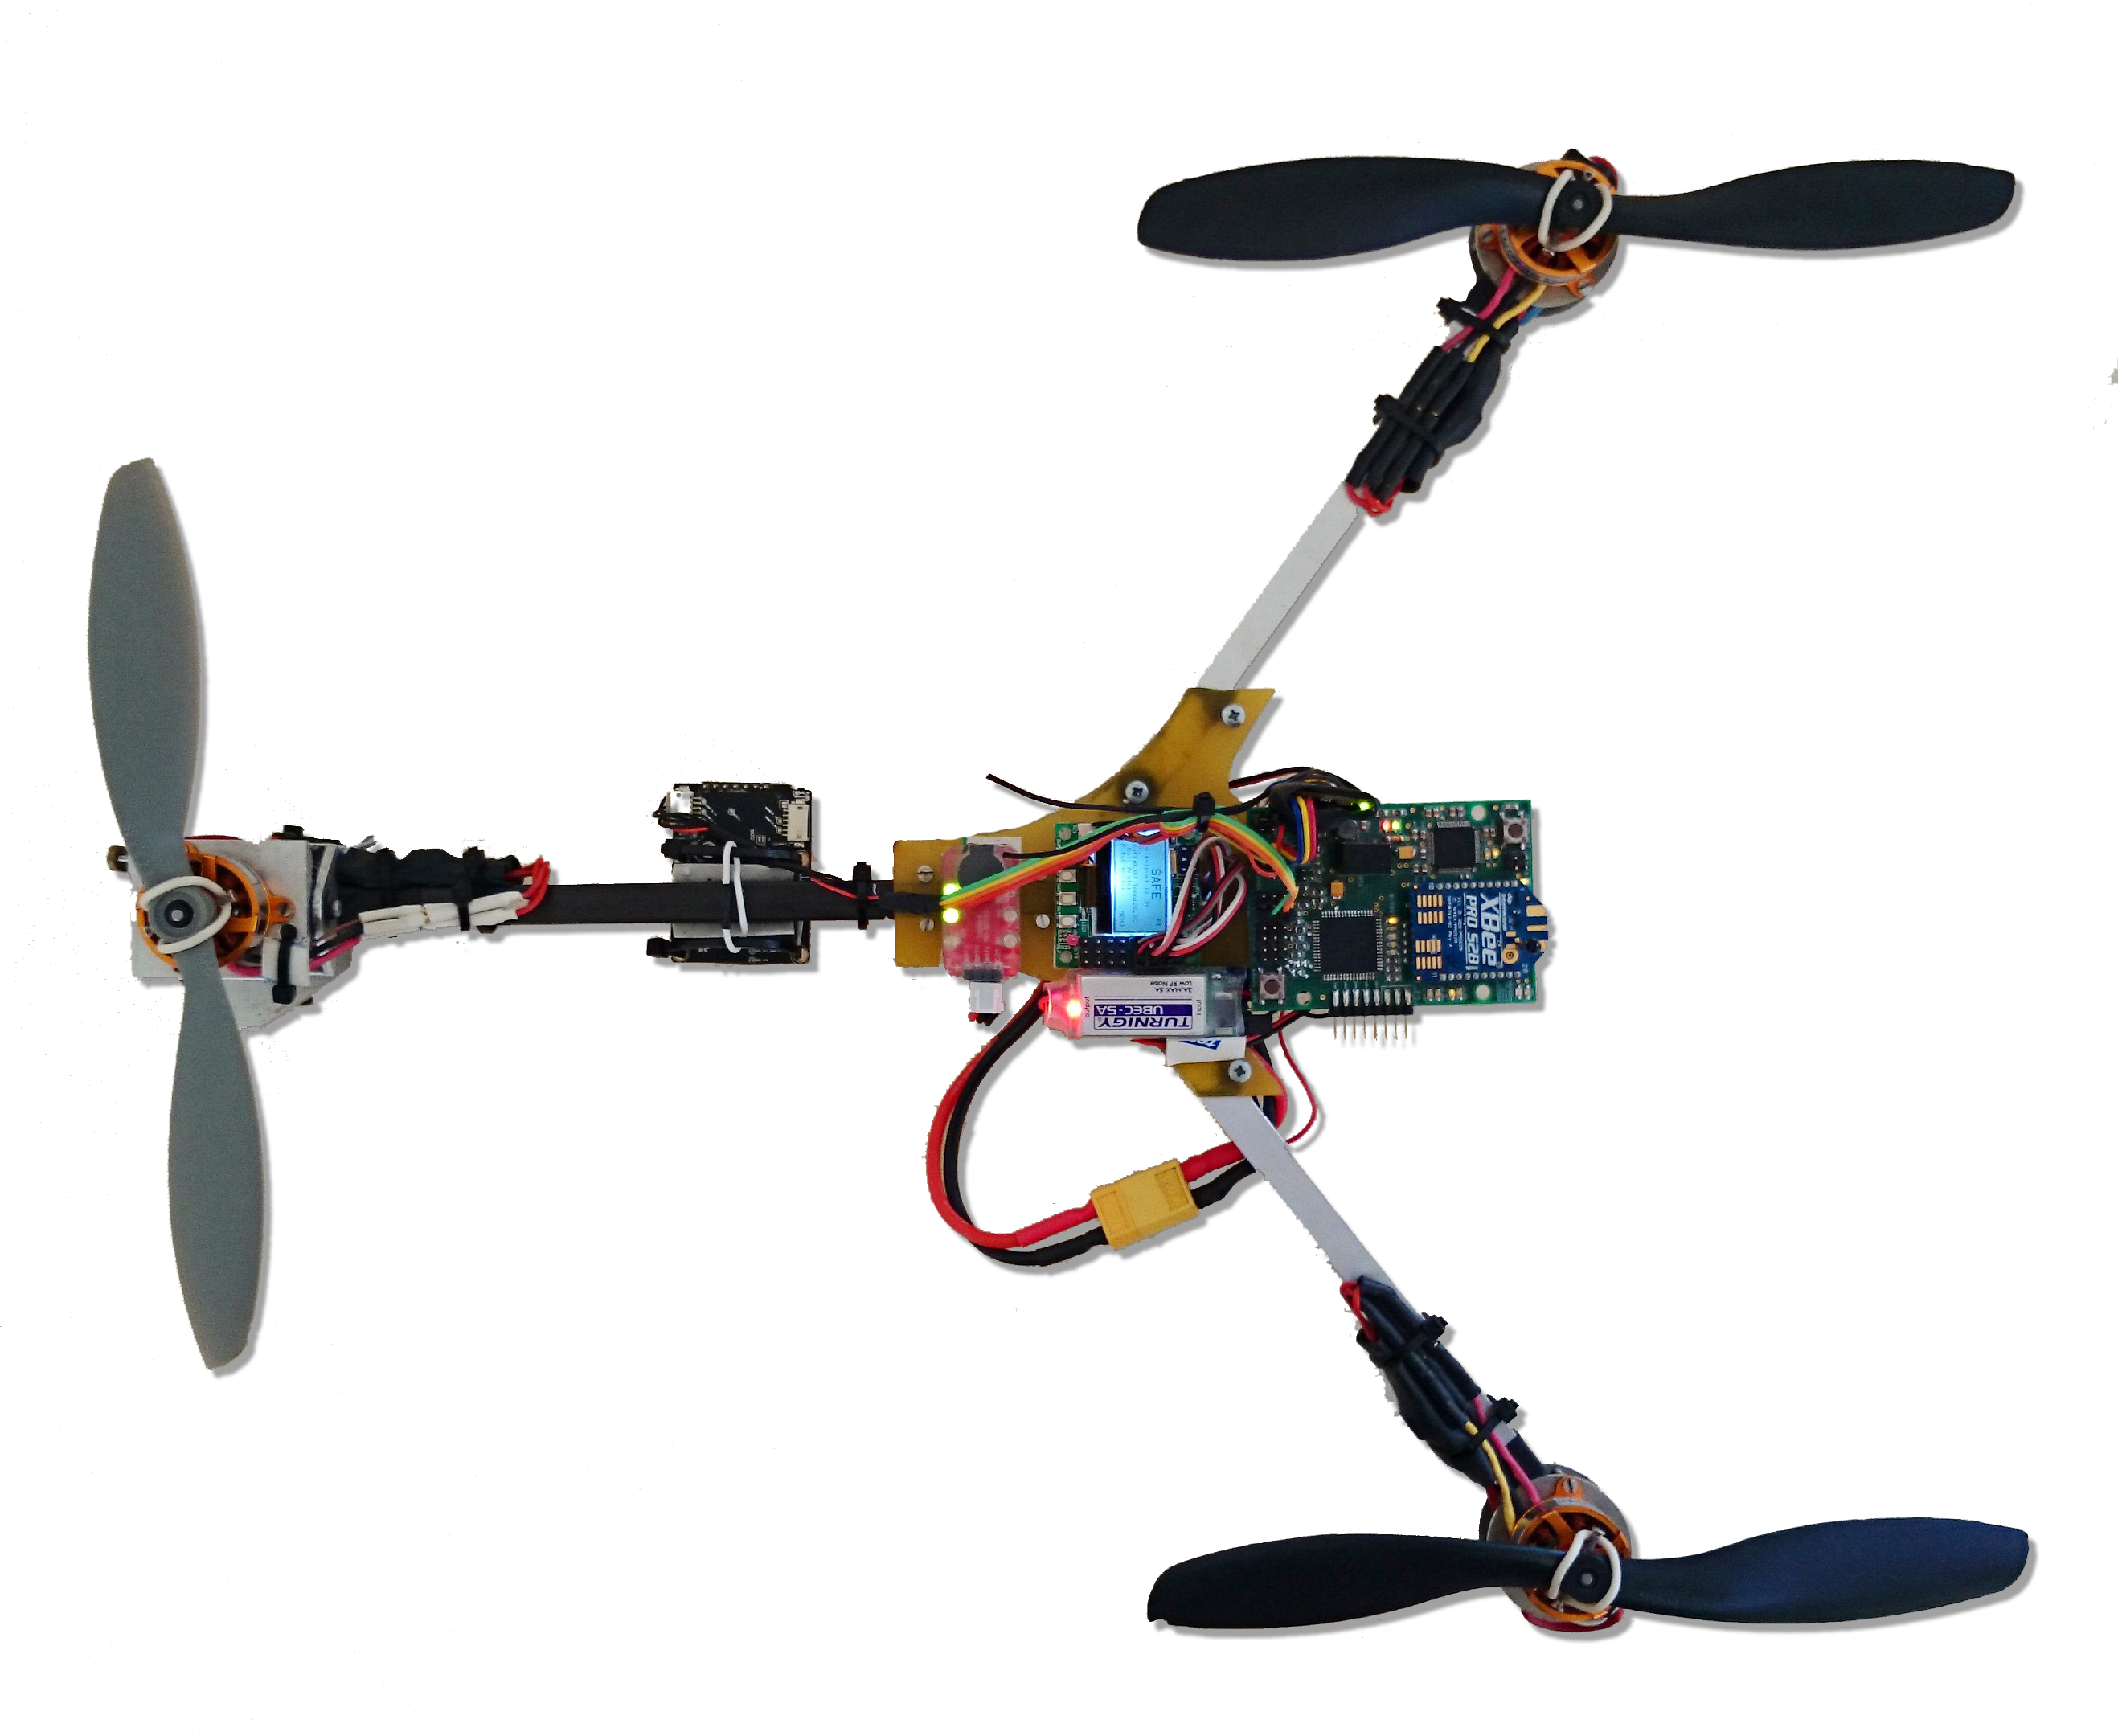
\includegraphics[width=\textwidth]{fig/tri1.jpg}
	\caption{Tricopter aircraft.}
	\label{fig:tricopter}
\end{subfigure}%
\begin{subfigure}[b]{0.45\textwidth}
	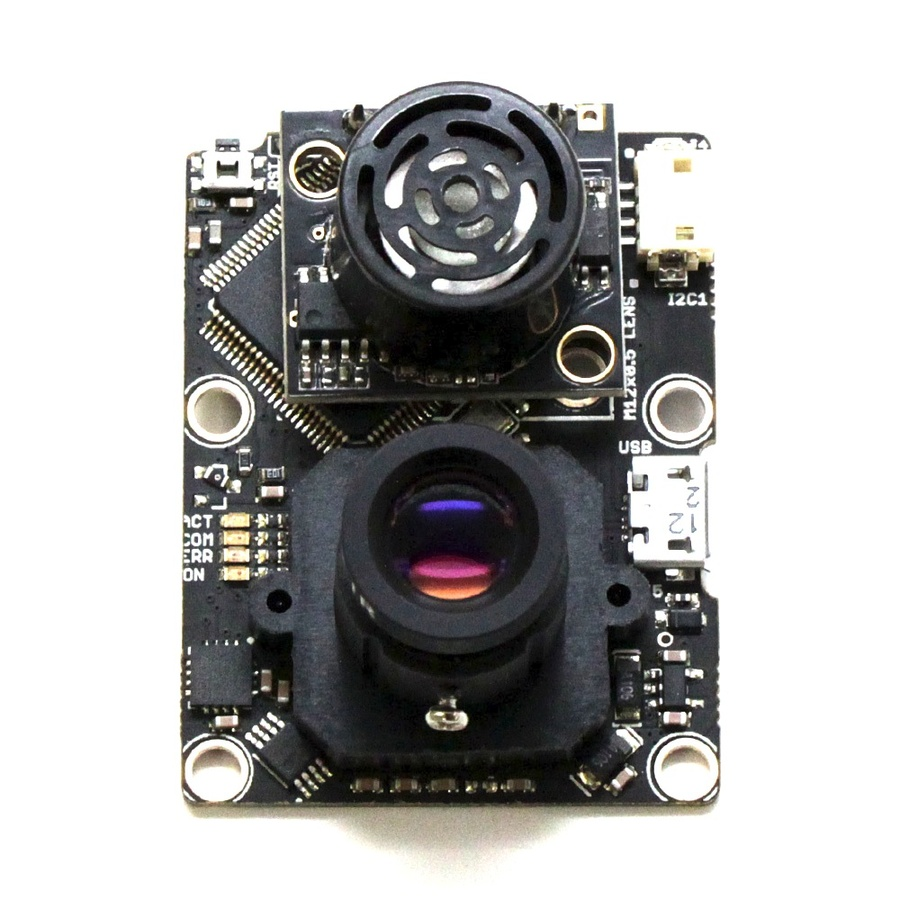
\includegraphics[width=\textwidth]{fig/px4flow.jpg}
	\caption{The px4flow sensor.}
	\label{fig:px4flow}
\end{subfigure}

\caption{Tricopter platform with px4flow optical flow sensor.}
\label{fig:tricopter_px4flow}
\end{figure}

\subsection{Custom control board v.2}

The control board v.2 (see fig. \ref{fig:custom_board}) is a significant improvement since the first version \citep{baca2013} which comprised only of a single 8-bit Atmel microcontroller. After 1 year of utilizing the old one, following requirements emerged that started a development of the second version. The platform should support variety of connections for external sensors and modules, mainly via UART and $\mathrm{i}^2\mathrm{c}$. It should support onboard data logging which is necessary for debugging and capturing data for system identification. Another requirement is a presence of a telemetry module. The UAV should be able to send short packets of data to another helicopter and to the ground station (laptop). The main motivation is to allow simple telemetry data being displayed on laptop while conducting an experiment. This should limit the success during experiments by offering a simple way to detect misbehaving sensors etc. Additionally there need to be a way to send simple commands from PC to the UAV. And the last and most important demand --- to support execution of the model predictive controller.

The board itself was built upon a standard (for UAVs) square mounting pattern ($45\times 45\jed{mm}$). It is designed in such way that allows mounting another board with dimensions $50\times 50\jed{mm}$ on top itself while not obscuring connectors, buttons and radio antenna. The board contains a $3.3\jed{V}, 1\jed{A}$ switching power supply that powers all its components. For an electrical schematic see Appendix~\ref{ape:schematic}, for layouts of the printed circuit board see Appendix~\ref{ape:pcb}. Following sections contain brief description of all key parts of the control board. Figure~\ref{fig:block_diagram_modules} shows a block diagram of all modules on the UAV.

\begin{figure}[htbp]
\centering

\begin{subfigure}[b]{0.515\textwidth}
	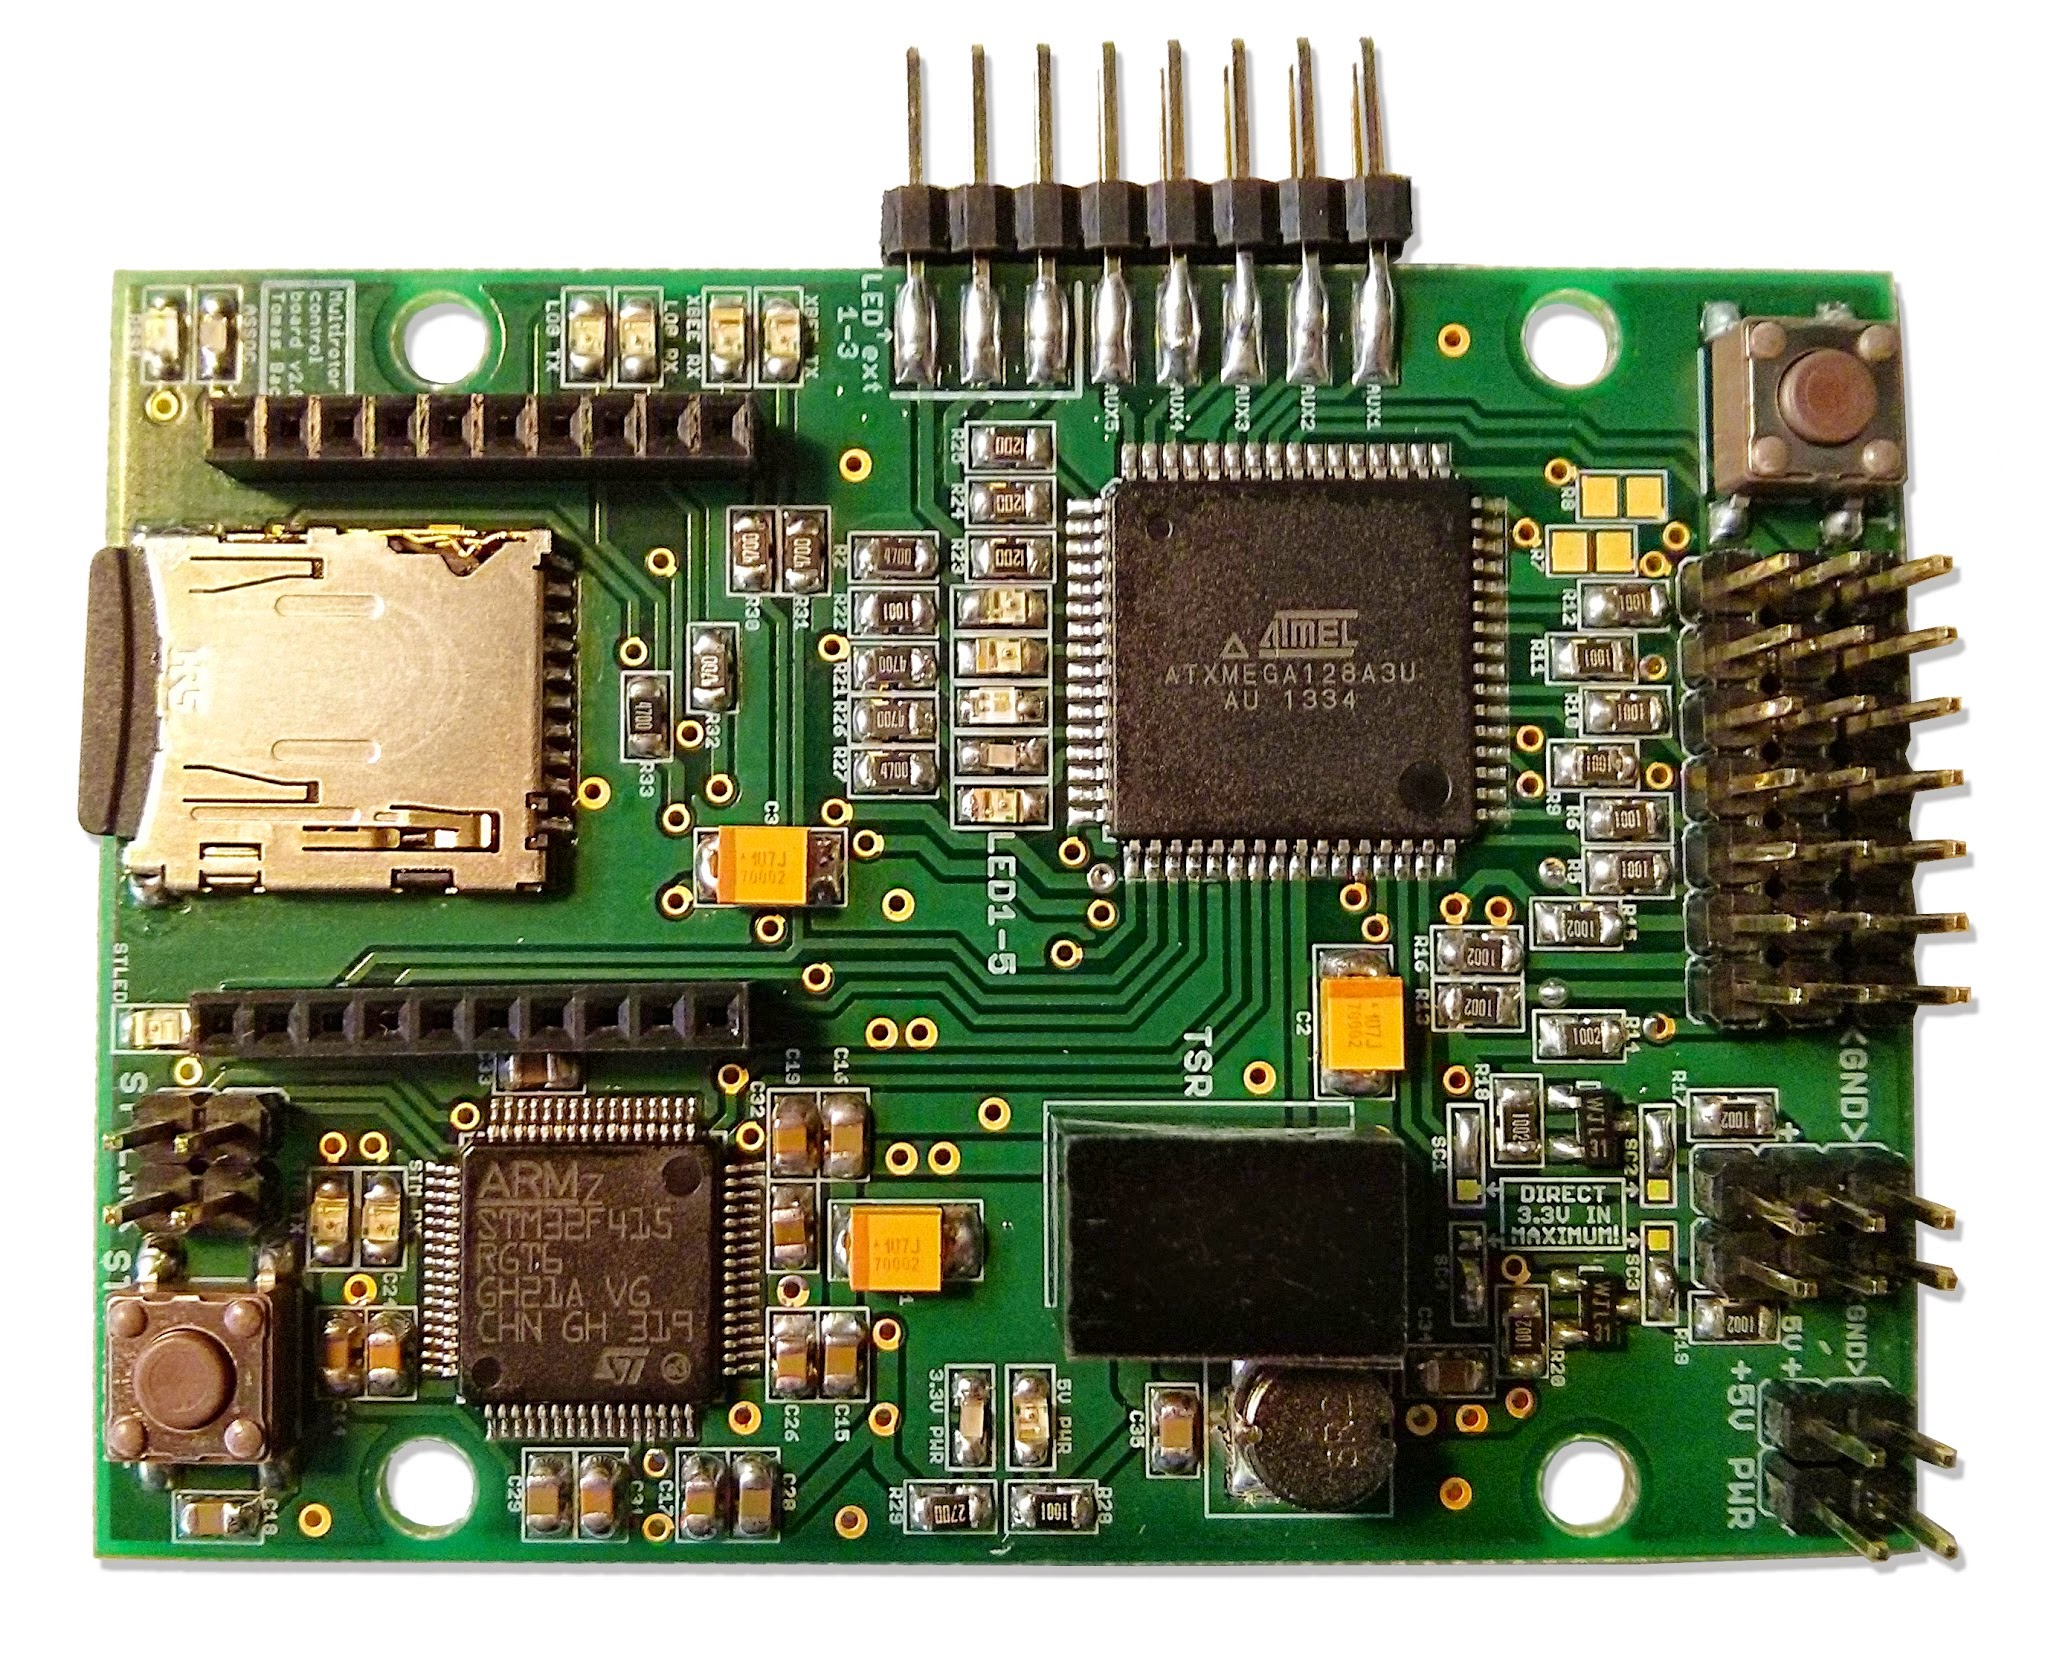
\includegraphics[width=\textwidth]{fig/board1.jpg}
	\caption{Board's top.}
	\label{fig:board_top}
\end{subfigure}%
\begin{subfigure}[b]{0.485\textwidth}
	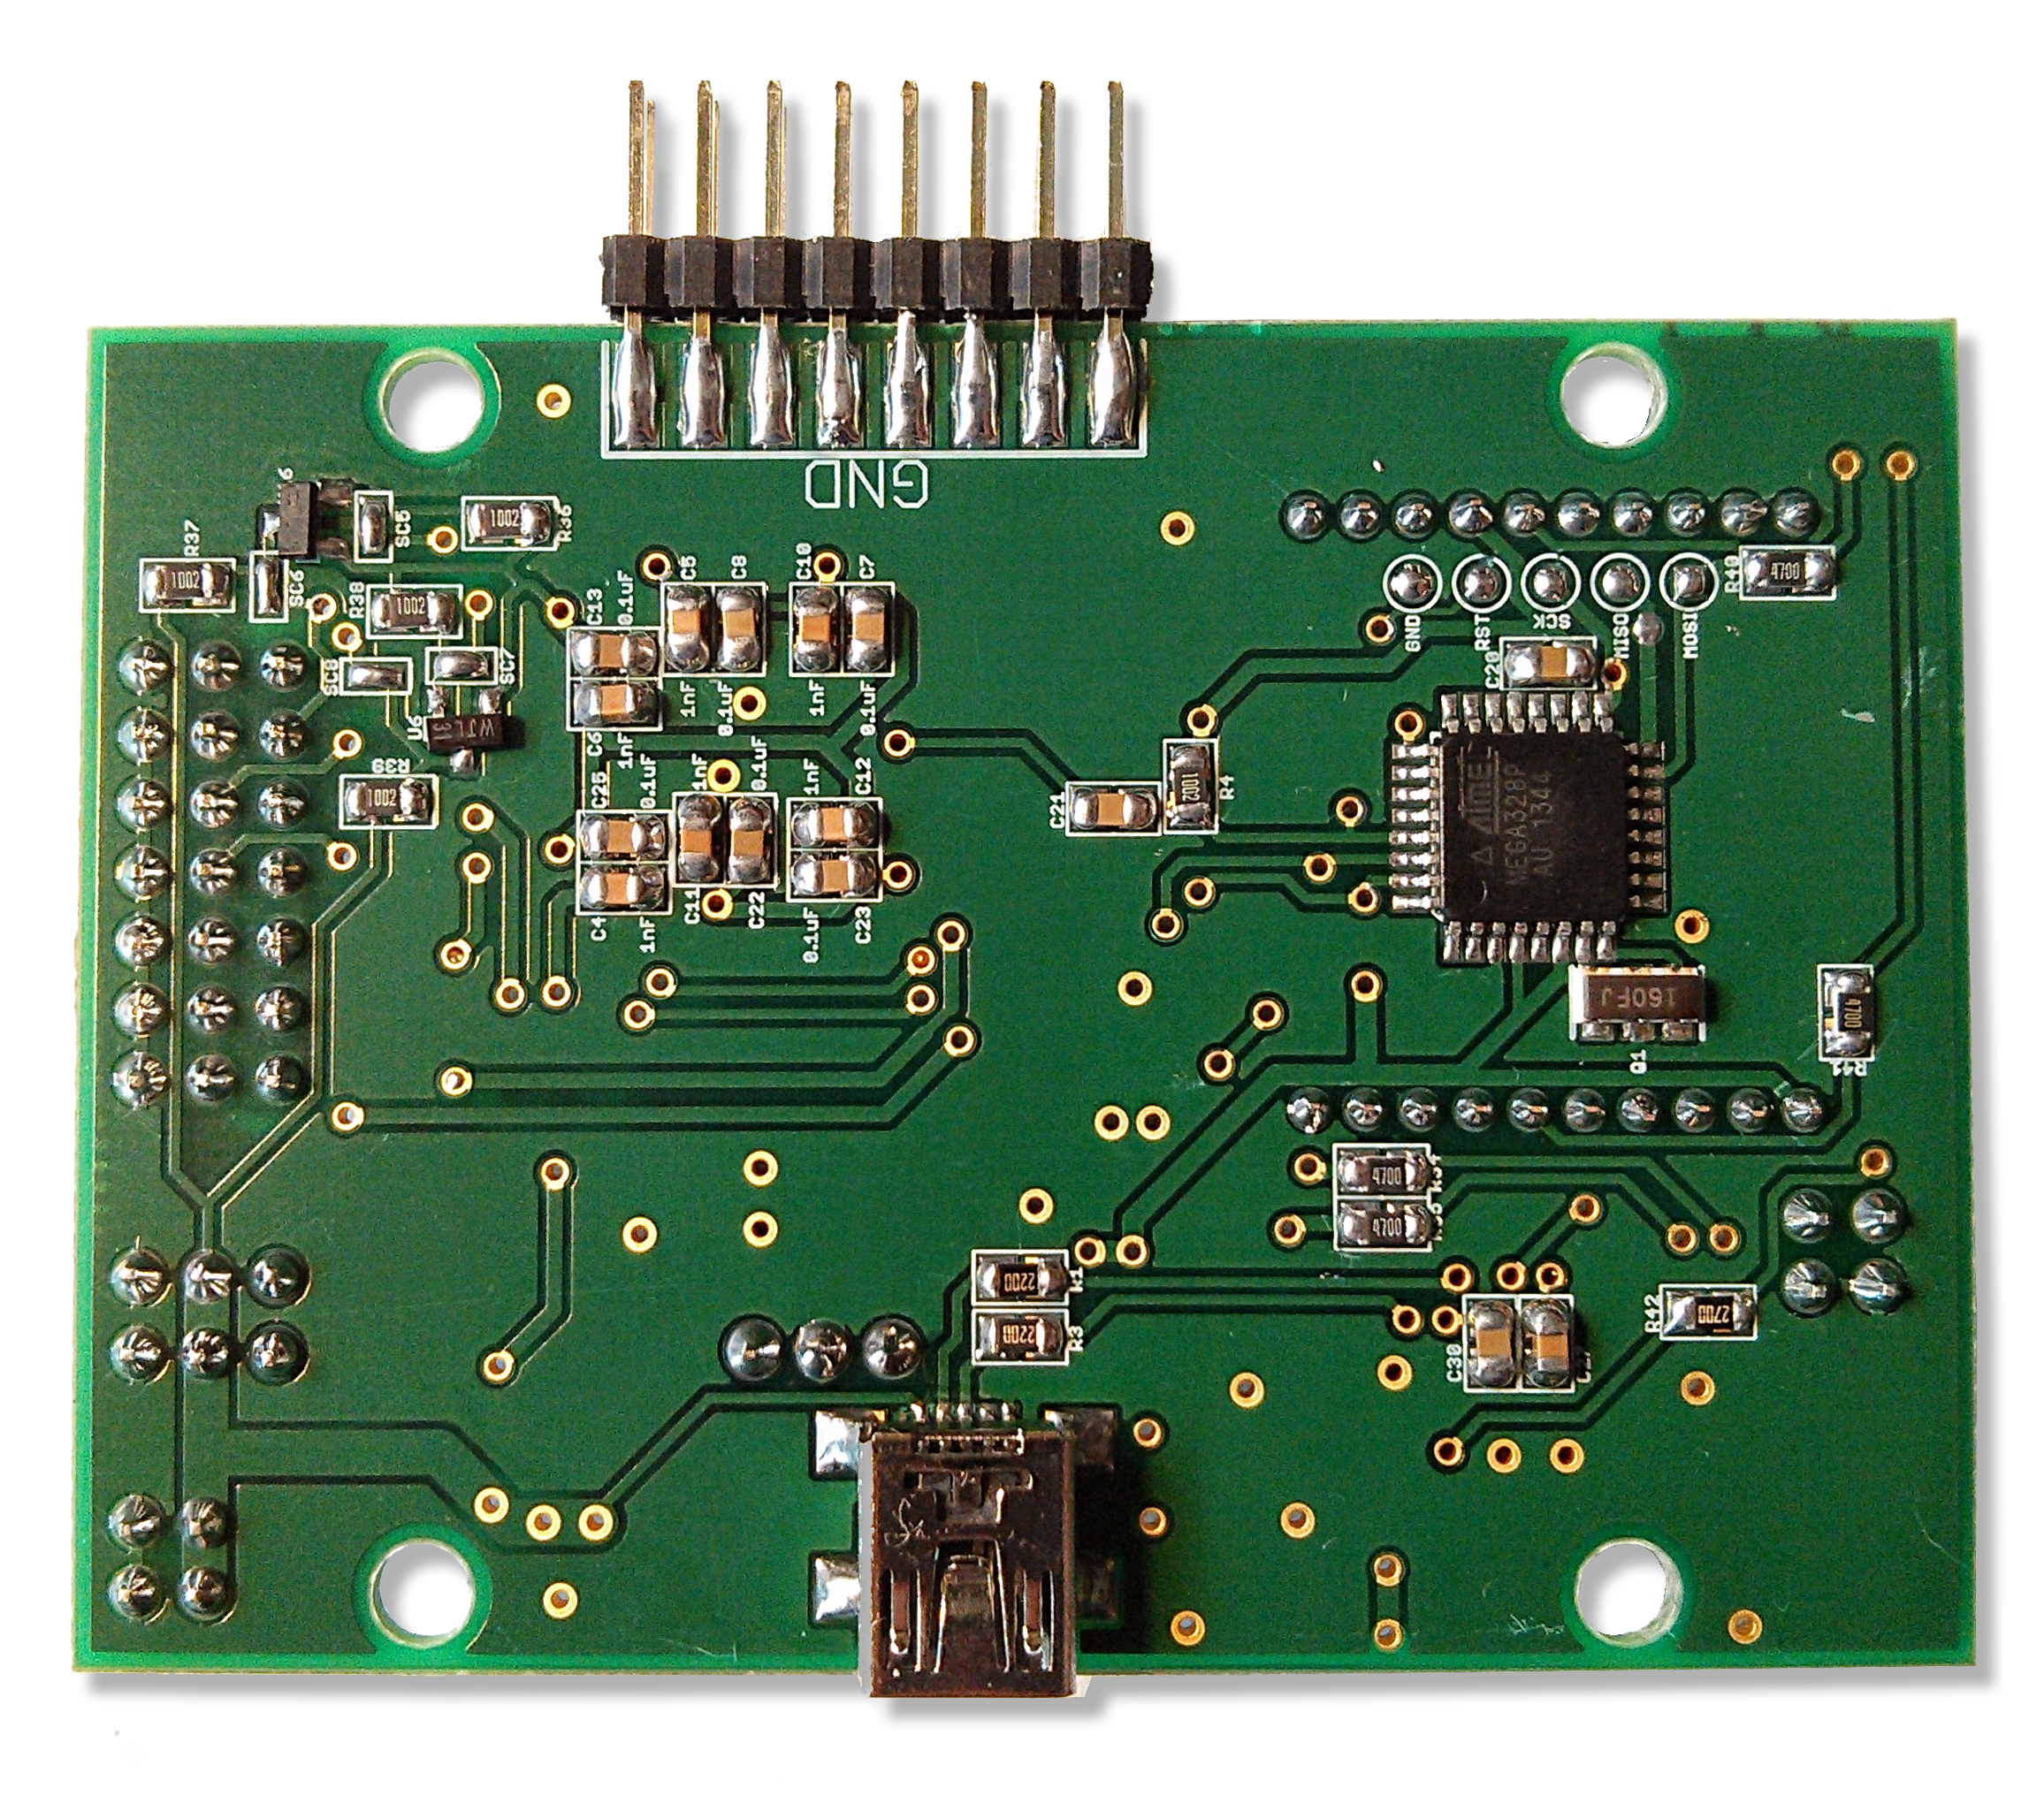
\includegraphics[width=\textwidth]{fig/board2.jpg}
	\caption{Board's bottom.}
	\label{fig:board_bottom}
\end{subfigure}

\caption{Custom control board v.2}
\label{fig:custom_board}
\end{figure}

\subsubsection{xMega main unit}

The first of two used microcontrollers is 8-bit AVR, ATxmega128a3u. It was decided to distribute software tasks (MPC, Kalman filter and others) onto two separate units. This MCU (microcontroller unit) is designated for handling all communication and other minor tasks. It is one of the most powerful MCUs in AVR 8-bit family with $32 \jed{MHz}$ clock and $8 \jed{kB}$ of SRAM memory. One of its biggest features are 7 separate UARTs. 3 of them are used for communication with other onboard parts, 4 of them are left free for connecting external devices. One is equipped with an optional level converter for connecting $5 \jed{V}$ devices. Additionally, there are two $\mathrm{i}^2\mathrm{c}$ lines and PPM\footnote{Pulse position modulation is a communication protocol commonly used on UAVs and RC models.} input/output for communicating with \textit{KK2} and RC receiver (both with optional level converters).

\subsubsection{ARM coprocessing unit}

The second MCU onboard is a powerful 32-bit ARM device produced by STMicroelectronics --- STM32F415RGT6. It is built upon ARM Cortex M4 with FPU (floating point unit) which allows a native work with floating point numbers. It has a powerful processor working on $168 \jed{MHz}$ accompanied by $192 \jed{kB}$ of RAM. This MCU is designated solely for computing Kalman filter and MPC. In is incorporated in such a way, that it only serves as an external coprocessor for xMega --- there are no peripherals connected to it. There are several reasons for choosing such architecture where the more powerful MCU does not server for all purposes although it has enough resources for it. The first one is the backwards compatibility with previously developed software. The xMega can execute it without many changes and it is also easier to develop on\footnote{The system as a whole is meant as a platform for another students to develop and test their work.}. Since the MPC and Kalman filter are important pieces of the program and their unwanted modification could make the machine dangerous, it was decided to conserve it on a separate MCU. The controller and KF are then used from the xMega MCU by a form of API. Important feature of STM is its floating point unit. Custom benchmarks has shown that it is capable of making $\approx 6 \times 10^6$ floating point operations per second which is a noticeable  difference comparing it to the xMega's $\approx 3\times 10^4$.

\subsubsection{XBee telemetry module}

When searching for a suitable wireless communication module, one can't miss the family of XBee devices \citep{xbee}. Built upon ZigBee standard, they can be set up to maintain one of several network topologies e.g. star or mesh. There are many different versions of XBee, based on its capabilities and frequency used. All of them support the same connection socket so they can be easily swapped for another type if necessary. Currently we use XBee Pro S2B which works on $2.4\jed{GHz}$ ISM band. Practical tests shown that it is not well suited for any real-time critical data transfers since there is a significant delay ($\approx 150\jed{ms}$)  and its throughput is $\approx 20\jed{kbit/s}$.

\subsubsection{OpenLog datalogging module}

Since we were not interested in creating our own data logger, we have implemented an existing, open source solution --- OpenLog \citep{openlog}. It has been designed to serve as an external SD card logging device connected by UART. Because its design is very simple, it was directly implemented into the control board. One can then set it up to receive a stream of data from the xMega MCU once the UAV is turned one. It can handle logging $30\jed{bytes}$ with rate $70\jed{Hz}$ which is sufficient for debugging and system identification.

\usetikzlibrary{shapes.geometric,backgrounds,calc}
\pgfdeclarelayer{background}
\pgfdeclarelayer{foreground}
\pgfsetlayers{background,main,foreground}

\begin{figure}[h]
\centering
\begin{tikzpicture}[->,>=stealth',node distance=1.5cm]

	\node[state] (atxmega) {
		\begin{tabular}{c}
  			ATxmega MCU\\

 		\end{tabular}
 	};
 	
	\node[state, right of = atxmega, shift = (right:2cm)] (stm) {
		\begin{tabular}{c}
  			ARM MCU\\
 		\end{tabular}
 	};
 	
	\node[state, above of = stm] (openLog) {
		\begin{tabular}{c}
  			OpenLog\\

 		\end{tabular}
 	};
 	
	\node[state, below of = stm] (XBee) {
		\begin{tabular}{c}
  			XBee\\

 		\end{tabular}
 	}; 
 
	\node[state, left of = atxmega, shift = (left:2.5cm)] (px4flow) {
		\begin{tabular}{c}
  			px4flow\\

 		\end{tabular}
 	}; 
 	
	\node[state, right of = XBee, shift = (right:2.5cm)] (pc) {
		\begin{tabular}{c}
  			Ground station\\

 		\end{tabular}
 	}; 
 	
	\node[state, above of = px4flow] (receiver) {
		\begin{tabular}{c}
  			RC receiver\\

 		\end{tabular}
 	}; 
 	
	\node[state, below of = px4flow] (kk2) {
		\begin{tabular}{c}
  			KK2 board\\

 		\end{tabular}
 	}; 

    \path (atxmega.north)+(1.4cm, 2.2cm) node (label1) {\textbf{Custom control board v.2}};
 
    \begin{pgfonlayer}{background}
    	\path (atxmega.west |- label1.north)+(-0.6,0.2) node (a) {};
        \path (XBee.south -| stm.east)+(+0.6,-0.5) node (b) {};
		\path[fill=gray!20, draw=black!50]
            (a) rectangle (b);
    \end{pgfonlayer}
       
	\path[->] ($(atxmega.north) + (+0.5cm, 0)$) edge [bend left=30] ($(openLog.west)$);
	\path[<->] (atxmega) edge (stm);
	\path[<->] ($(atxmega.south) + (+0.5cm, 0)$) edge [bend right=30] ($(XBee.west)$);
	\path[->] (px4flow) edge (atxmega);
	\path[->] ($(receiver.east)$) edge [bend left=30] ($(atxmega.north) + (-0.5cm, 0)$);
	\path[<->,dashed] (XBee) edge (pc);
	\path[<-] ($(kk2.east)$) edge [bend right=30] ($(atxmega.south) + (-0.5cm, 0)$);

\end{tikzpicture}
\caption{Block diagram of modules on the UAV.}
\label{fig:block_diagram_uav}
\end{figure}

\subsection{FreeRTOS and tasks}

When creating a program for MCU such as xMega and STM, one can basically choose between two ways of doing that. The most straightforward is to develop the bare application that will be directly executed on the processor while utilizing all of its computational resources. It is up to the creator of the program to manage concurrent processes, interact with hardware and supply fast communication responses in parallel with long-running calculations. In previous work, the software was developed exactly in that way. Its benefit is obvious. The programmer has a complete control over the hardware --- it is only his code being executed on the CPU. But when the application gets complicated, an operating system can be used to take care of allocating computational resources for different parts of the program. There is a family of operating systems intended for real-time application such as the ours --- Real-Time Operating Systems (RTOS). 

The reader should not confuse the RTOS with the notion of operating system usually used on personal computers. These are special software developed with different criteria. The main one is its scheduling which ensures each application is given its time slot in a deterministic and defined time. It usually works based on hardware timers and interrupts. Context switch in RTOS is usually very fast and it happens relatively often to allow real-time processing of incoming data. One of widely used RTOS is the FreeRTOS \citep{freertos}. An Open Source solution with existing ports for both MCUs used in the control board. It offers a capability to create so called \textit{tasks}, an analogy of processes in classical operating systems. Tasks are separate pieces of program with its own CPU context and memory stack. 

The RTOS takes care of switching between tasks based on given priority allowing user to develop apparently multitask application. There are new issues coming with this concept --- the problem of synchronization and sharing resources. The FreeRTOS incorporates \textit{queues} and \textit{semaphores} which are supposed to be used for exchanging data between tasks and for their synchronization. We have implemented the FreeRTOS on both MCUs creating separate tasks for handling communication and computations. See figure \ref{fig:block_diagram_uav} for view on tasks and the information flow between them.

Since our system requires executing controllers and estimators in rates in order of tens\jed{Hz} and it has to handle communication in rate in order of hundreds\jed{Hz} the context switch rate was chosen in order of magnitude faster --- $1000\jed{Hz}$. But still there are operations that require even faster execution and reaction times (e.g. reception and creation of pulse-position signal or buffering raw data from peripherals). That is why here remains a part of the control software executed directly on interrupt basis, independently of the FreeRTOS. Because safety is the great concern of us, the system is able to hand over the UAV to the human operator even when the FreeRTOS and the control system does not work properly or even freezes. Both implementations on our MCUs requires around $4\jed{kB}$ of memory leaving out enough for custom code.

\subsection{Tasks on xMega MCU}

The software on xMega consists of 4 different tasks running equally in parallel. There is \emph{CommTask} which is designated to handle all incoming and outgoing communication. Since 	sharing access to all communication media would be difficult to maintain, all other tasks communicate with peripherals via the CommTask. Another one is \emph{ControllersTask} which handles computations with regards to system controllers. \emph{LogTask} is responsible for periodic data logging to OpenLog module. And despite its name, \emph{MainTask} handles minor jobs as trajectory following and flight state automaton (modeling different flight modes of the UAV). 

\subsection{Tasks on STM MCU}

Tasks on STM has much clearer designation. There is also the \emph{CommTask} serving as a communication mediator. The another one is \emph{KalmanTask}. It handles the complete computation of the Kalman filter. Finally the last one is \emph{MPCTask} that takes care of computing the model predictive controller. 

\begin{figure}[h]	
\centering
\begin{tikzpicture}[->,>=stealth',node distance=1.5cm]

	\node[state] (commtask) {
		\begin{tabular}{c}
  			CommTask\\
 		\end{tabular}
 	};
 	
	\node[state, left of = commtask, shift = (left:2.4cm)] (controllerstask) {
		\begin{tabular}{c}
  			ControllersTask\\
 		\end{tabular}
 	};
 	
	\node[state, above of = commtask, shift = (left:2.1cm)] (maintask) {
		\begin{tabular}{c}
  			MainTask\\
 		\end{tabular}
 	};

	\node[state, below of = commtask, shift = (left:2.1cm)] (logtask) {
		\begin{tabular}{c}
  			LogTask\\
 		\end{tabular}
 	};
 	
	\node[state, right of = commtask, shift = (right:3cm)] (commtask2) {
		\begin{tabular}{c}
  			CommTask\\
 		\end{tabular}
 	};

	\node[state, above of = commtask2, shift = (right:2.6cm)] (kalmantask) {
		\begin{tabular}{c}
  			KalmanTask\\
 		\end{tabular}
 	};
 	
	\node[state, below of = commtask2, shift = (right:2.6cm)] (mpctask) {
		\begin{tabular}{c}
  			MPCTask\\
 		\end{tabular}
 	};

	\path (maintask.north)+(0cm, 0.5cm) node (label1) {\textbf{xMega MCU}};
	\path (kalmantask.north)+(-1cm, 0.5cm) node (label2) {\textbf{STM MCU}};
 
    \begin{pgfonlayer}{background}
    	\path (controllerstask.west |- label1.north)+(-0.6,0.2) node (a) {};
        \path (logtask.south -| commtask.east)+(+0.6,-0.5) node (b) {};
		\path[fill=gray!20, draw=black!50]
            (a) rectangle (b);
    \end{pgfonlayer}
    
    \begin{pgfonlayer}{background}
    	\path (commtask2.west |- label2.north)+(-0.6,0.2) node (a) {};
        \path (mpctask.south -| kalmantask.east)+(+0.6,-0.5) node (b) {};
		\path[fill=gray!20, draw=black!50]
            (a) rectangle (b);
    \end{pgfonlayer}
       
	\path[<->] (maintask) edge [bend left] ($(commtask.north)$);
	\path[<->] (commtask) edge (controllerstask);
	\path[<->] (controllerstask) edge [bend left] (maintask);
	\path[<->] (commtask) edge (commtask2);
	\path[<->] (commtask2) edge [bend left] (kalmantask);
	\path[->] (kalmantask) edge [bend left=45] (mpctask);
	\path[<->] (mpctask) edge [bend left] (commtask2);
	\path[->] ($(commtask.south)$) edge [bend left] (logtask);

\end{tikzpicture}
\caption{Block diagram of information flow between tasks of xMega and STM MCUs.}
\label{fig:block_diagram_modules}
\end{figure}

\subsection{CMatrixLib - ANSI C matrix library}

In order to implement the Kalman filter (section \ref{cap:kalman_filter_theory}) and the model predictive controller (section \ref{cap:mpc_theory}) one has to deal mainly with vector and matrix operations. Although it can be implemented directly using the programming language, it is impractical for code debugging and it discards the clarity of mathematical matrix notation. There is a large selection of matrix libraries \citep{matrixlibraries} available for variety of programming languages. But since both our code projects are developed using ANSI C programming language and our platforms are specific (the library should be supplied by means of its source code) we decided to develop our own matrix library. Another reason that supports this decision is to maintain as much control over the executed code as possible, specifically with regards to memory allocation, which is a critical issue on microcontrollers (and considering we are dealing with matrices and vectors with dimensions in order of hundreds). Our library supports basic matrix and vector operations with floating point values as well as basic algebra operators --- matrix inversion and computation of determinant. It was developed with regard to minimize memory stack footprint by requiring prior memory allocation for subresults. There is also a possibility to create a matrix using a constant data located within the program memory. CMatrixLib, as we named it, is released on a community website GitHub \citep{cmatrixlib} under GNU General Public License together with a proper documentation.

\subsection{Summary}

This section presents the platform used for development, testing and evaluation of model predictive controller onboard the UAV. The aircraft is of classical tricopter design utilizing built-in stabilization board. We proposed a custom control board for handling signal processing and controller computation onboard while supplying wireless telemetry and data logging. Two different microcontrollers were used to allow a decomposition of the code --- computationally intensive tasks (Kalman filter and MPC) are located on 32-bit ARM coprocessor while communication and other tasks are left on 8-bit xMega MCU. Both systems utilize FreeRTOS, Real-Time operating system. RTOS Tasks were presented with brief description of their purpose. In order to implement KF and MPC on these microcontrollers, a CMatrixLib matrix library was developed and published as an Open Source project. 